\documentclass[12pt]{article}
\usepackage[pdftex]{graphicx}
%\usepackage[body={190mm,277mm},top=10mm,left=10mm,nohead]{geometry}

%\documentclass[12pt]{article}
%\usepackage[utf8]{inputenc} % nastavuje pou�it� k�dov�n�, u�ivatel� Windows zam�n� latin2 za cp1250
%\usepackage[T1]{fontenc}
\usepackage{a4wide} % nastavuje standardn� evropsk� form�t str�nek A4
%%\usepackage{index} % nutno pou��t v p��pad� tvorby rejst��ku bal��kem makeindex
%%\usepackage{fancybox} % umo��uje pokro�il� r�me�kov�n� :-)
%\usepackage[pdftex]{graphicx} % nezbytn� pro standardn� vkl�d�n� obr�zk� do dokumentu
%\usepackage{enumerate}
%\usepackage{listings}
%\usepackage[dvips]{color}
\usepackage{subfigure}
%\usepackage{amssymb,amsmath

\setlength{\parindent}{0pt} 
\setlength{\parskip}{2ex}

\title{Solution for assignment \#1}
\date{October 27, 2012}
\author{Vojtech Kopal}

\newcommand{\mytilde}{\raise.17ex\hbox{$\scriptstyle\mathtt{\sim}$} }

\begin{document}

\maketitle

\clearpage

\section{Economic part}

\subsection*{a) Economic growth and convergence - descriptive statistics:}

\begin{figure}[h!]
  \centering           
  \subfigure{                         
  	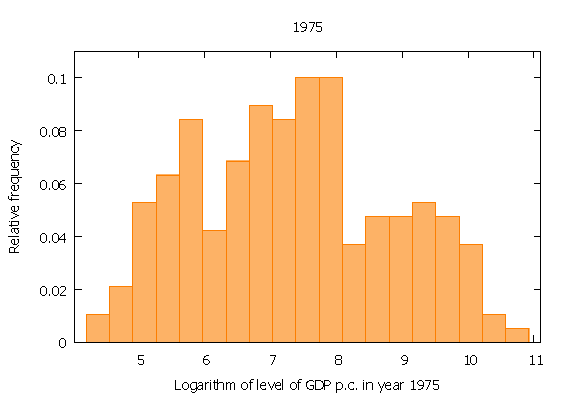
\includegraphics[scale=0.7]{parts/1a_1}
  	\label{1a:gpd1975}
  }                   
  \subfigure{                         
  	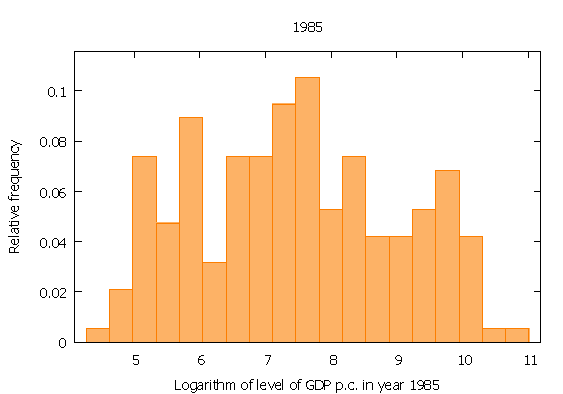
\includegraphics[scale=0.7]{parts/1a_2}
  	\label{1a:gpd1985}
  }                 
  \subfigure{                         
  	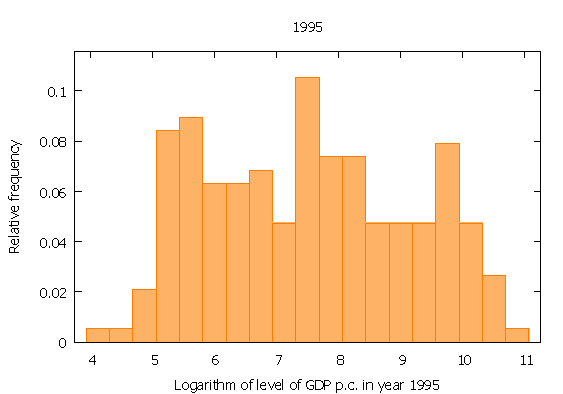
\includegraphics[scale=0.7]{parts/1a_3}
  	\label{1a:gpd1995}
  }                 
  \subfigure{                         
  	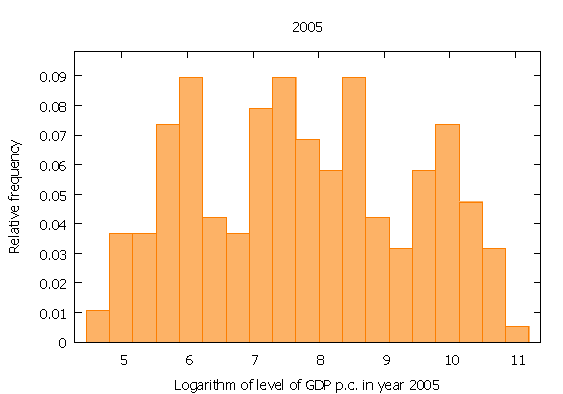
\includegraphics[scale=0.7]{parts/1a_4}
  	\label{1a:gpd2005}
  }                         
  \caption{The changes in distribution of GDP p.c. among 190 countries in years 1975, 1985, 1995 and 2005.}
\end{figure}

Omitting Djibouti.

Commenting on changes.

\clearpage

Median income in 1975 is 1487.6

Rich countries

\begin{figure}[h!]
  \centering           
  \subfigure{                         
  	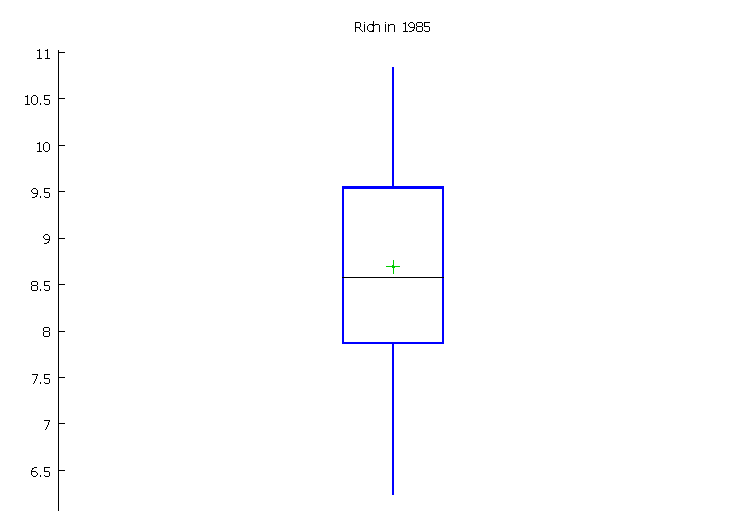
\includegraphics[scale=0.3]{parts/1a_5}
  	\label{1a:rich1985}
  }                   
  \subfigure{                         
  	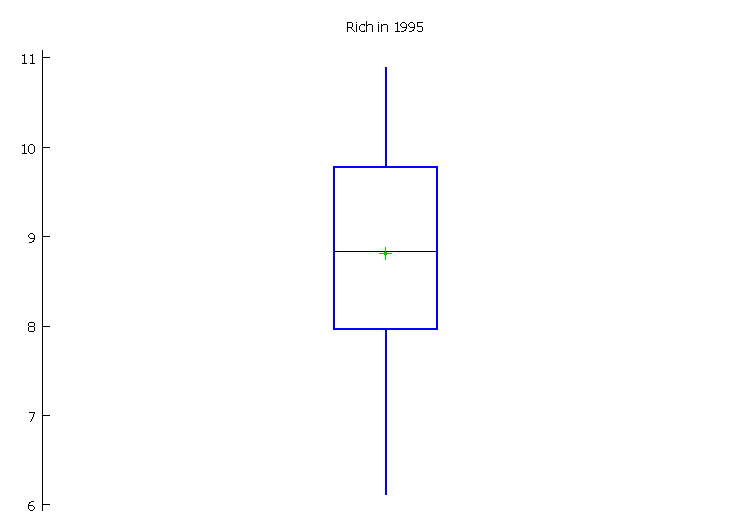
\includegraphics[scale=0.3]{parts/1a_6}
  	\label{1a:rich1995}
  }                 
  \subfigure{                         
  	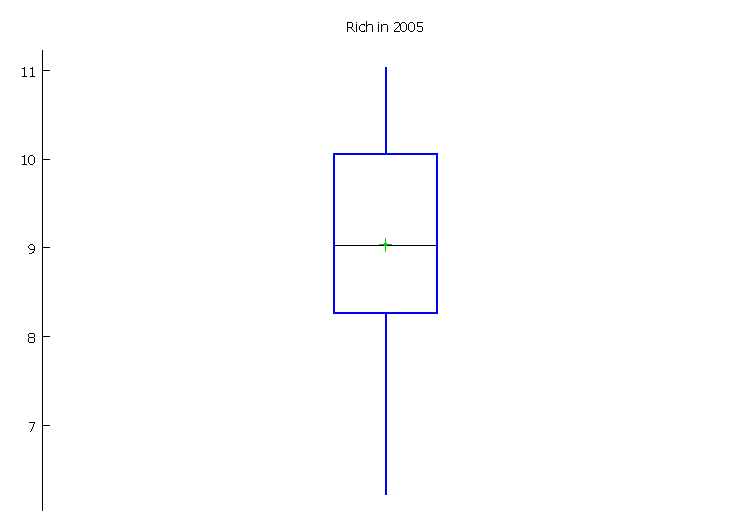
\includegraphics[scale=0.3]{parts/1a_7}
  	\label{1a:rich2005}
  }                        
  \caption{Development of income for rich countries in years 1985, 1995, 2005.}
\end{figure}

Poor countries

\begin{figure}[h!]
  \centering           
  \subfigure{                         
  	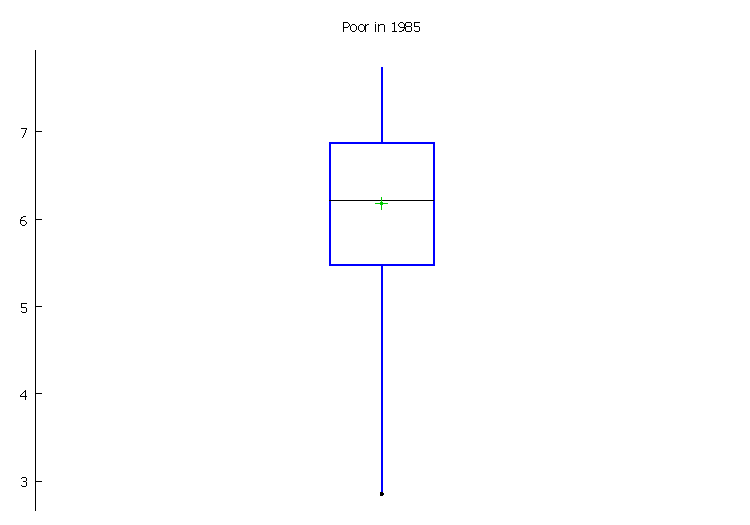
\includegraphics[scale=0.3]{parts/1a_8}
  	\label{1a:poor1985}
  }                   
  \subfigure{                         
  	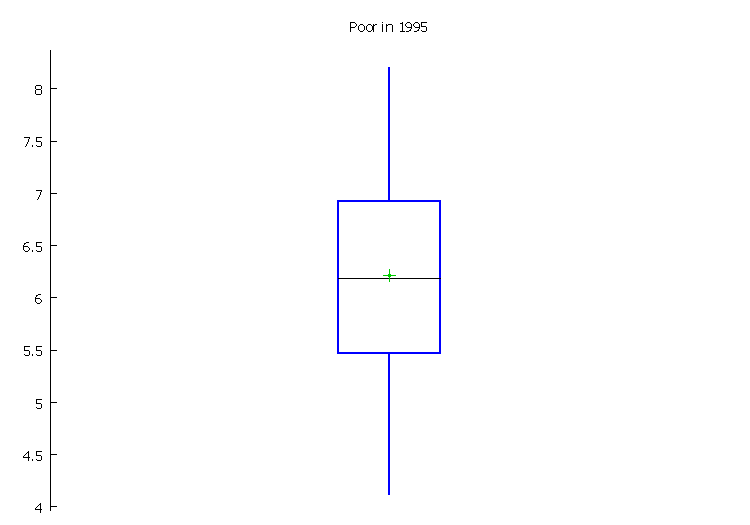
\includegraphics[scale=0.3]{parts/1a_9}
  	\label{1a:poor1995}
  }                 
  \subfigure{                         
  	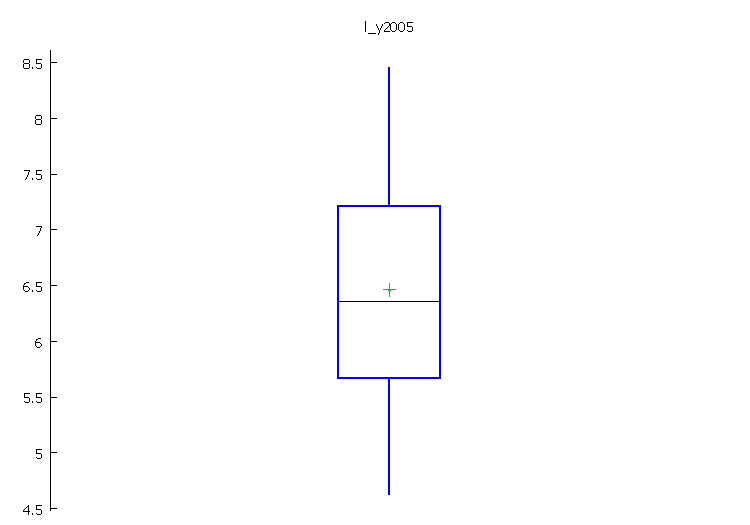
\includegraphics[scale=0.3]{parts/1a_10}
  	\label{1a:poor2005}
  }                        
  \caption{Development of income for poor countries in years 1985, 1995, 2005.}
\end{figure}

\subsection*{b) The Solow model:}

\section{Reading+Essay}

The article has analyzed how different countries with advanced economies dealt with a public debt over last 100 years. The question was whether any of the recipes that have been used is applicable also in today's situation. An observed episode starts with a debt-to-GDP ratio of a country getting over 100 \% and such episode lasts for following 15 years. There is 26 of such identified high-debt episodes between years 1875 and 2012.

Main conclusions drawn from the historical experience follows.

Fiscal changes have to be structural with long-term prospects. It is necessary to approach for primary surplus. A good example was the path of Canada from a primary deficit to a surplus, which goal was needed to support the rest of consolidation. As it can be seen from observed episodes, it takes quite a long time to get there. As it is mentioned in article, it is rare to have an improvement of 1 \% per year on average over a long-term period.
 
The structural and long-term changes are not only about fiscal policies, but they are also required in case of weak banking system and corporate sector. In Japan such issues undermined effectiveness of monetary policy which resulted in poor result in fiscal consolidation.

If those long-term and structural approach are chosen rather than temporary measures, it is ideal environment to start the long run to reduced debt while low real rates and loose monetary conditions.
 
As case studies six following countries have been chosen: the United Kingdom, the United States, Belgium, Italy, Japan and Canada. I will explain the implication on Belgium. For me there are two phase in Belgium's struggling with debt. In the first they have set up structural changes in social system: they have reduced finances going into welfare payments, family allowances, unemployment insurance, etc. They have also reduced number of people employed in public sector. This first phase failed when fiscal efforts faced monetary conditions aiming at maintaining the peg for European Currency Unit and recession in 1990. After that the debt-to-GDP ratio again got over 100 \% up to 134 \% in 1993. Luckily for Belgium the long-term structural changes with combination with a new second plan (starting from 1990) allowed Belgium to reduce budget deficit to less than 3 \% and thus meet the Maastricht criteria by 1997. The second plan contained additional tax increases and spending cuts.

To sum up, thanks to first phase Belgium managed to overcome recession period 1990 - 1993 and by continuing with second plan (tax increases and additional cuts) they have lowered the public debt almost by 50 \% between years 1993 and 2007. This case study shows how important is to combine fiscal consolidation with the right monetary environment with low real rates. Also when compared with Italy, which has similar environment, when dealing with debt I can see that structural reforms allows faster debt reduction comparing to only temporal solutions, which have been made in Italy. I should also mention that another booster when lowering public debts is strong external demand, which also helped Belgium.

By this article I have been introduced to an issue how to deal with public debts. However, sooner or later the observed countries could have tuned the monetary policy such that it was supportive to on-going fiscal consolidations. What am I missing here and what should be worth further analysis is how should countries which are parts of a monetary union, e.g. eurozone, proceed when dealing with a public debt. 

\end{document}